% ===================== I. Motivation =====================
\section{Motivation}

% Slide 3
\begin{frame}{From parton distributions to 3D tomography}
  \begin{columns}[c]
    \begin{column}{0.40\textwidth}
      \begin{itemize}
        \item Deep inelastic scattering: a quark carries the light-cone momentum fraction
        \[ x = \frac{k^+}{P^+} \]
        \item Collinear PDFs $f_1(x)$ are a \textbf{1D} picture.
        \item \textbf{TMDs} keep the transverse momentum $\vprp{k}$: momentum-space tomography.
        \item TMDs need semi-inclusive processes (SIDIS, Drell--Yan).
      \end{itemize}
    \end{column}
    \begin{column}{0.58\textwidth}
      \centering
      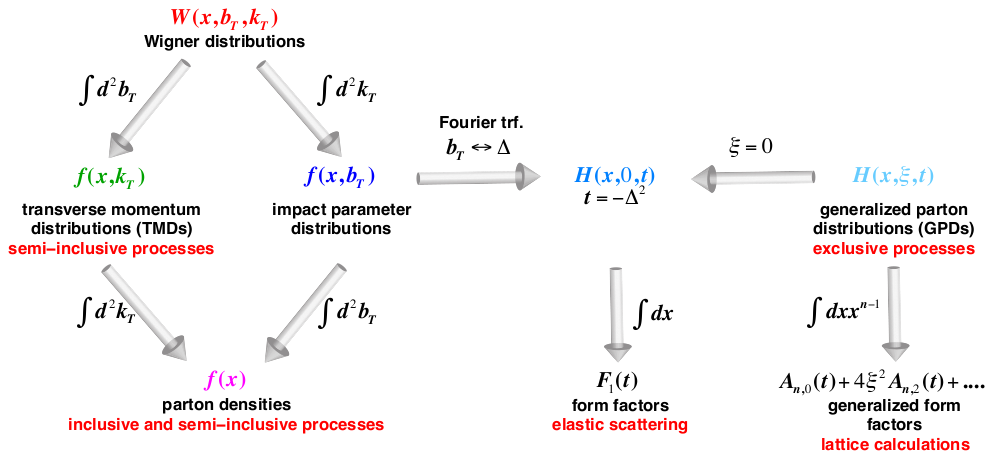
\includegraphics[width=\linewidth]{EIC_WP_Fig2p2_distributions.png}
      \figsrc{Adapted from Accardi \emph{et al.}, EPJA \textbf{52}, 268 (2016)}
    \end{column}
  \end{columns}
\end{frame}

\begin{frame}{Transverse position and transverse momentum}
  \begin{columns}[c]
  \begin{column}{0.55\textwidth}
  \begin{itemize}
    \item GPDs encode transverse position, through Fourier transformation of transverse momentum transfer $\vect\Delta_T$.
    \item TMDs encode the quark transverse momentum $\vect k_T$.
    \item The impact parameter in this picture is distinct from the quark-field separation $\vect b_T$ used in the TMD correlator.
  \end{itemize}
  \[ \rho_q(x,\vect b_T)=\int\frac{d^2\vect\Delta_T}{(2\pi)^2}
       e^{-i\vect b_T\cdot\vect\Delta_T}H^q(x,0,-\vect\Delta_T^2). \]
  \end{column}
  \begin{column}{0.41\textwidth}\centering
    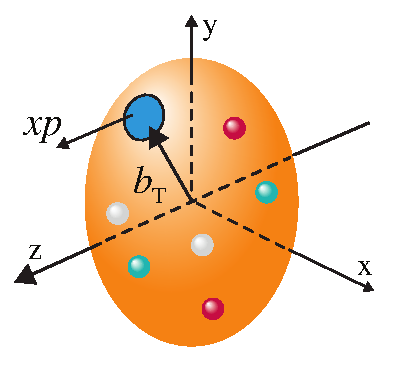
\includegraphics[width=\linewidth,height=0.65\textheight,keepaspectratio]{EIC_WP_Fig2p1_parton_bT.pdf}
  \end{column}
  \end{columns}
  \figsrc{Thesis, Ch. 2; Accardi et al., EPJA 52, 268 (2016), arXiv:1212.1701, Fig. 2.1 (CC BY 4.0).}
\end{frame}

\begin{frame}{Leading-twist quark TMDs}
  \centering\renewcommand{\arraystretch}{1.65}
  \begin{tabular}{c|ccc}
    Nucleon $\backslash$ quark & unpolarized & longitudinal & transverse\\\hline
    Unpolarized & $f_1$ & & $h_1^\perp$ (T-odd)\\
    Longitudinal & & $g_1$ & $h_{1L}^\perp$\\
    Transverse & $f_{1T}^\perp$ (T-odd) & $g_{1T}$ & $h_1,\ h_{1T}^\perp$
  \end{tabular}
  \vspace{4mm}
  \begin{itemize}
    \item The Sivers function describes unpolarized quarks in a transversely polarized nucleon.
    \item Sivers and Boer--Mulders functions change sign between future- and past-pointing staple links.
  \end{itemize}
  \figsrc{Thesis, Ch. 2: leading-twist quark TMD polarization table.}
\end{frame}

% Slide 4
\begin{frame}{Single-spin asymmetries and the Sivers effect}
  \begin{columns}[c]
    \begin{column}{0.48\textwidth}
      \begin{itemize}
        \item Large left--right asymmetries off transversely polarized protons (E704, 1991).
        \item Leading-twist collinear hard-scattering estimates predict tiny asymmetries (Kane, Pumplin, Repko 1978).
        \item Sivers (1990): the quark $\vprp{k}$ distribution is \textbf{shifted perpendicular to the spin}.
      \end{itemize}
      \vspace{-1mm}
      \[ f_{q/N^\uparrow}(x,\vprp{k}) = f_1^q(x,\vprp{k}^2) - \frac{\epsilon_{ij}\,k_{T,i}\,S_{T,j}}{\mN}\, f_{1T}^{\perp q}(x,\vprp{k}^2) \]
      \centering
      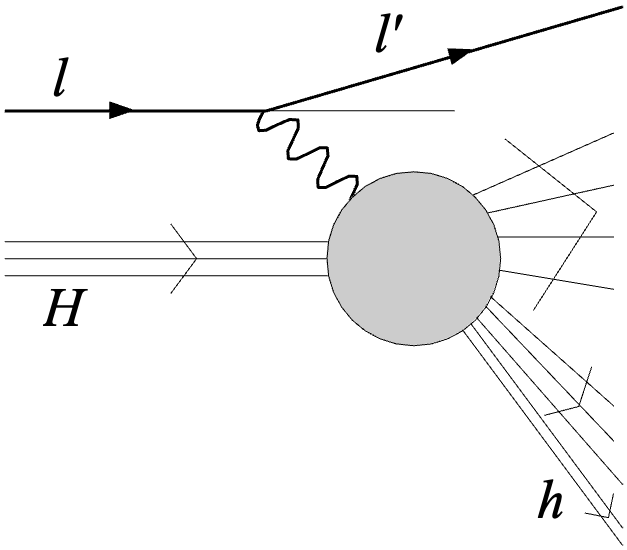
\includegraphics[width=0.42\linewidth]{SIDIS.png}\\
      {\tiny SIDIS: $\ell N^\uparrow\to\ell' h X$}
    \end{column}
    \begin{column}{0.50\textwidth}
      \centering
      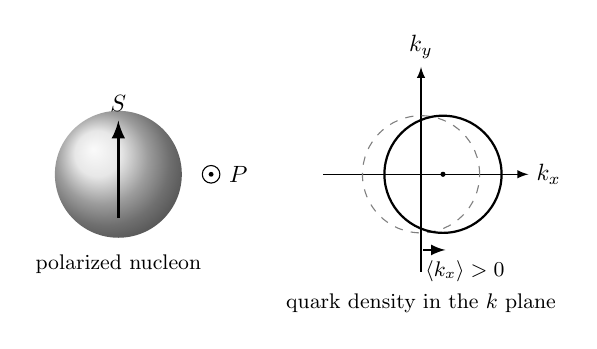
\begin{tikzpicture}[scale=0.62, every node/.style={scale=0.85}]
        \begin{scope}[shift={(-3.2,0)}]
          \shade[ball color=gray!25] (0,0) circle (1.3);
          \draw[very thick, -latex] (0,-0.9) -- (0,1.1) node[above] {$\vprp{S}$};
          \draw (1.9,0) circle (0.18); \fill (1.9,0) circle (0.05);
          \node[right] at (2.1,0) {$\vect{P}$};
          \node at (0,-1.85) {\small polarized nucleon};
        \end{scope}
        \begin{scope}[shift={(3.0,0)}]
          \draw[-latex] (-2.0,0) -- (2.2,0) node[right] {$k_x$};
          \draw[-latex] (0,-2.0) -- (0,2.2) node[above] {$k_y$};
          \draw[dashed, gray] (0,0) circle (1.2);
          \draw[thick] (0.45,0) circle (1.2);
          \fill (0.45,0) circle (1.5pt);
          \draw[-latex, thick] (0.05,-1.55) -- (0.5,-1.55);
          \node[below] at (0.9,-1.6) {\small $\langle k_x\rangle > 0$};
          \node at (0,-2.65) {\small quark density in the $\vprp{k}$ plane};
        \end{scope}
      \end{tikzpicture}
      \\[1mm]
      {\scriptsize $\vect{P}$ out of the page, $\vprp{S}\parallel\hat y$: the shift is along $\hat x$ (shown: $f_{1T}^\perp<0$).\\
      In the Sivers-shift definition $\vprp{S}\parallel\hat x$ and we measure $\langle k_y\rangle$.}
    \end{column}
  \end{columns}
\end{frame}

% Slide 5
\begin{frame}{Why it is not zero: the gauge link}
  \begin{itemize}
    \item Collins (1993): neglecting the process-dependent gauge link led to a vanishing Sivers function.
    \item Brodsky--Hwang--Schmidt (2002): final-state interactions give a nonzero asymmetry.
    \item Collins (2002): a gauge-invariant TMD needs a \textbf{Wilson line}. Its path depends on the process, and T-reversal swaps the two paths:
  \end{itemize}
  \[ f_{1T}^{\perp}(x,\vprp{k}^2)\Big|_{\text{SIDIS}} = - f_{1T}^{\perp}(x,\vprp{k}^2)\Big|_{\text{DY}} \]
  \centering
  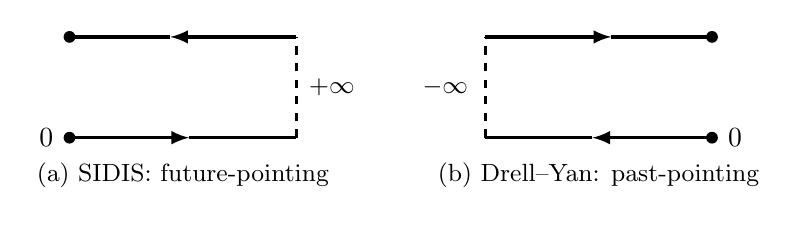
\begin{tikzpicture}[scale=0.8, q/.style={circle, fill=black, inner sep=1.5pt}]
    \begin{scope}[shift={(0,0)}]
      \node[q, label=left:{$0$}] at (0,0) {};
      \node[q, label=left:{$\bvec$}] at (0,1.6) {};
      \draw[very thick, -latex] (0,0) -- (1.9,0);
      \draw[very thick] (1.9,0) -- (3.6,0);
      \draw[very thick, dashed] (3.6,0) -- (3.6,1.6);
      \draw[very thick, -latex] (3.6,1.6) -- (1.6,1.6);
      \draw[very thick] (1.6,1.6) -- (0,1.6);
      \node[right] at (3.65,0.8) {\small $+\infty\,\nminus$};
      \node at (1.8,-0.6) {\small (a) SIDIS: future-pointing};
    \end{scope}
    \begin{scope}[shift={(10.2,0)}]
      \node[q, label=right:{$0$}] at (0,0) {};
      \node[q, label=right:{$\bvec$}] at (0,1.6) {};
      \draw[very thick, -latex] (0,0) -- (-1.9,0);
      \draw[very thick] (-1.9,0) -- (-3.6,0);
      \draw[very thick, dashed] (-3.6,0) -- (-3.6,1.6);
      \draw[very thick, -latex] (-3.6,1.6) -- (-1.6,1.6);
      \draw[very thick] (-1.6,1.6) -- (0,1.6);
      \node[left] at (-3.65,0.8) {\small $-\infty\,\nminus$};
      \node at (-1.8,-0.6) {\small (b) Drell--Yan: past-pointing};
    \end{scope}
  \end{tikzpicture}
  \keymsg{We put this \textbf{staple-shaped link} on the lattice.}
\end{frame}

% Slide 7
\begin{frame}{The $x$-gap on the lattice, and this thesis}
  \begin{columns}[c]
    \begin{column}{0.52\textwidth}
      \begin{itemize}
        \item Light-like separations cannot be placed at a single Euclidean time.
        \item Lorentz-invariant amplitude method with staple links (Musch \emph{et al.} 2012): first lattice Sivers shift and its sign change.
        \item The earlier staple-link Sivers-shift calculations used here sit at $\bvec\tcdot P=0$. Since $\bvec\tcdot P$ is Fourier-conjugate to $x$, they are \textbf{$x$-integrated}.
        \item SIDIS measurements constrain the Sivers function. The combined COMPASS Drell--Yan data are consistent with its predicted sign change; extracting the $x$-shape requires phenomenological fits.
      \end{itemize}
    \end{column}
    \begin{column}{0.46\textwidth}
      \centering
      \begin{tikzpicture}[scale=0.9]
        \draw[-latex, thick] (-3,0) -- (3.2,0) node[right] {$\bvec\tcdot P$};
        \fill[badred] (0,0) circle (3pt);
        \node[badred, above, align=center, font=\footnotesize] at (0,0.15) {earlier work:\\$\bvec\tcdot P=0$ $\Rightarrow\int dx$};
        \draw[okgreen, line width=4pt, opacity=0.6] (-2.4,-0.45) -- (2.4,-0.45);
        \node[okgreen!70!black, below, font=\footnotesize, align=center] at (0,-0.6) {this thesis: scan $\bvec\tcdot P\neq0$,\\Fourier transform $\Rightarrow$ function of $x$};
      \end{tikzpicture}
    \end{column}
  \end{columns}
\figsrc{Musch et al., Phys. Rev. D 85, 094510 (2012); COMPASS, Phys. Rev. Lett. 133, 071902 (2024), arXiv:2312.17379.}
\end{frame}
\begin{frame}{The extraction procedure}
  \vspace{2mm}
  \begin{block}{This thesis}
    \begin{enumerate}
      \item Kinematic constraint at $\bvec\tcdot P\neq0$ $\Rightarrow$ off-axis staples, built by interpolation.
      \item Map the data to $(\bvec\tcdot P,\ \bvec^2)$, keeping $|\vect b|\ge 3a$.
      \item Find a model that can be Fourier transformed: a power law, fit to all amplitudes at once.
      \item Fourier transform to $x$, extrapolate to the light-cone limit, test factorization.
    \end{enumerate}
  \end{block}
\figsrc{Thesis, Chs. 5--7: extraction, candidate selection, Fourier transformation and extrapolation.}
\end{frame}
